% Created by tikzDevice version 0.12.3 on 2020-04-10 11:41:05
% !TEX encoding = UTF-8 Unicode
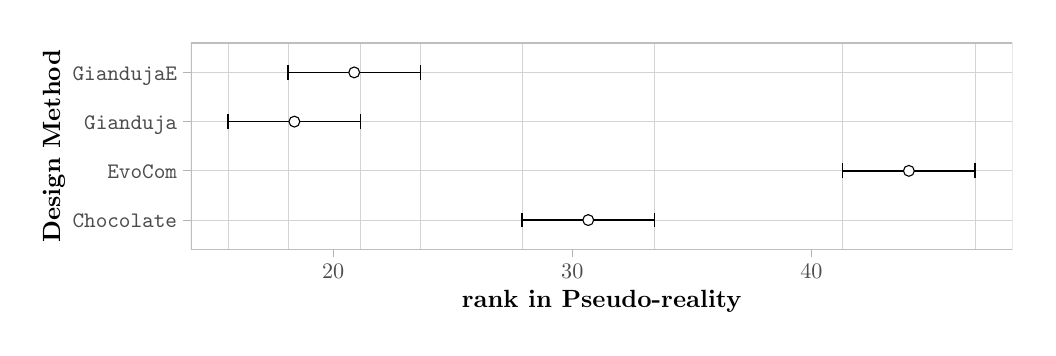
\begin{tikzpicture}[x=1pt,y=1pt]
\definecolor{fillColor}{RGB}{255,255,255}
\path[use as bounding box,fill=fillColor,fill opacity=0.00] (0,0) rectangle (361.35,108.41);
\begin{scope}
\path[clip] (  0.00,  0.00) rectangle (361.35,108.41);
\definecolor{drawColor}{RGB}{255,255,255}
\definecolor{fillColor}{RGB}{255,255,255}

\path[draw=drawColor,line width= 0.6pt,line join=round,line cap=round,fill=fillColor] (  0.00,  0.00) rectangle (361.35,108.41);
\end{scope}
\begin{scope}
\path[clip] ( 58.95, 28.23) rectangle (355.85,102.91);
\definecolor{fillColor}{RGB}{255,255,255}

\path[fill=fillColor] ( 58.95, 28.23) rectangle (355.85,102.91);
\definecolor{drawColor}{RGB}{211,211,211}

\path[draw=drawColor,line width= 0.3pt,line join=round] ( 58.95, 56.67) --
	(355.85, 56.67);

\path[draw=drawColor,line width= 0.3pt,line join=round] ( 58.95, 74.46) --
	(355.85, 74.46);

\path[draw=drawColor,line width= 0.3pt,line join=round] ( 58.95, 92.24) --
	(355.85, 92.24);

\path[draw=drawColor,line width= 0.3pt,line join=round] ( 58.95, 38.89) --
	(355.85, 38.89);

\path[draw=drawColor,line width= 0.2pt,line join=round] (226.50, 28.23) -- (226.50,102.91);

\path[draw=drawColor,line width= 0.2pt,line join=round] (342.35, 28.23) -- (342.35,102.91);

\path[draw=drawColor,line width= 0.2pt,line join=round] (120.32, 28.23) -- (120.32,102.91);

\path[draw=drawColor,line width= 0.2pt,line join=round] (141.93, 28.23) -- (141.93,102.91);

\path[draw=drawColor,line width= 0.2pt,line join=round] (178.63, 28.23) -- (178.63,102.91);

\path[draw=drawColor,line width= 0.2pt,line join=round] (294.48, 28.23) -- (294.48,102.91);

\path[draw=drawColor,line width= 0.2pt,line join=round] ( 72.45, 28.23) -- ( 72.45,102.91);

\path[draw=drawColor,line width= 0.2pt,line join=round] ( 94.05, 28.23) -- ( 94.05,102.91);
\definecolor{drawColor}{RGB}{0,0,0}

\path[draw=drawColor,line width= 0.6pt,line join=round] (226.50, 36.23) --
	(226.50, 41.56);

\path[draw=drawColor,line width= 0.6pt,line join=round] (226.50, 38.89) --
	(178.63, 38.89);

\path[draw=drawColor,line width= 0.6pt,line join=round] (178.63, 36.23) --
	(178.63, 41.56);

\path[draw=drawColor,line width= 0.6pt,line join=round] (342.35, 54.01) --
	(342.35, 59.34);

\path[draw=drawColor,line width= 0.6pt,line join=round] (342.35, 56.67) --
	(294.48, 56.67);

\path[draw=drawColor,line width= 0.6pt,line join=round] (294.48, 54.01) --
	(294.48, 59.34);

\path[draw=drawColor,line width= 0.6pt,line join=round] (120.32, 71.79) --
	(120.32, 77.12);

\path[draw=drawColor,line width= 0.6pt,line join=round] (120.32, 74.46) --
	( 72.45, 74.46);

\path[draw=drawColor,line width= 0.6pt,line join=round] ( 72.45, 71.79) --
	( 72.45, 77.12);

\path[draw=drawColor,line width= 0.6pt,line join=round] (141.93, 89.57) --
	(141.93, 94.90);

\path[draw=drawColor,line width= 0.6pt,line join=round] (141.93, 92.24) --
	( 94.05, 92.24);

\path[draw=drawColor,line width= 0.6pt,line join=round] ( 94.05, 89.57) --
	( 94.05, 94.90);

\path[draw=drawColor,line width= 0.4pt,line join=round,line cap=round,fill=fillColor] (202.56, 38.89) circle (  1.96);

\path[draw=drawColor,line width= 0.4pt,line join=round,line cap=round,fill=fillColor] (318.42, 56.67) circle (  1.96);

\path[draw=drawColor,line width= 0.4pt,line join=round,line cap=round,fill=fillColor] ( 96.38, 74.46) circle (  1.96);

\path[draw=drawColor,line width= 0.4pt,line join=round,line cap=round,fill=fillColor] (117.99, 92.24) circle (  1.96);
\definecolor{drawColor}{RGB}{190,190,190}

\path[draw=drawColor,line width= 0.6pt,line join=round,line cap=round] ( 58.95, 28.23) rectangle (355.85,102.91);
\end{scope}
\begin{scope}
\path[clip] (  0.00,  0.00) rectangle (361.35,108.41);
\definecolor{drawColor}{gray}{0.30}

\node[text=drawColor,anchor=base east,inner sep=0pt, outer sep=0pt, scale=  0.80] at ( 54.00, 53.92) {\texttt{EvoCom}};

\node[text=drawColor,anchor=base east,inner sep=0pt, outer sep=0pt, scale=  0.80] at ( 54.00, 71.70) {\texttt{Gianduja}};

\node[text=drawColor,anchor=base east,inner sep=0pt, outer sep=0pt, scale=  0.80] at ( 54.00, 89.48) {\texttt{GiandujaE}};

\node[text=drawColor,anchor=base east,inner sep=0pt, outer sep=0pt, scale=  0.80] at ( 54.00, 36.14) {\texttt{Chocolate}};
\end{scope}
\begin{scope}
\path[clip] (  0.00,  0.00) rectangle (361.35,108.41);
\definecolor{drawColor}{gray}{0.70}

\path[draw=drawColor,line width= 0.3pt,line join=round] ( 56.20, 56.67) --
	( 58.95, 56.67);

\path[draw=drawColor,line width= 0.3pt,line join=round] ( 56.20, 74.46) --
	( 58.95, 74.46);

\path[draw=drawColor,line width= 0.3pt,line join=round] ( 56.20, 92.24) --
	( 58.95, 92.24);

\path[draw=drawColor,line width= 0.3pt,line join=round] ( 56.20, 38.89) --
	( 58.95, 38.89);
\end{scope}
\begin{scope}
\path[clip] (  0.00,  0.00) rectangle (361.35,108.41);
\definecolor{drawColor}{gray}{0.70}

\path[draw=drawColor,line width= 0.3pt,line join=round] (110.38, 25.48) --
	(110.38, 28.23);

\path[draw=drawColor,line width= 0.3pt,line join=round] (196.80, 25.48) --
	(196.80, 28.23);

\path[draw=drawColor,line width= 0.3pt,line join=round] (283.23, 25.48) --
	(283.23, 28.23);
\end{scope}
\begin{scope}
\path[clip] (  0.00,  0.00) rectangle (361.35,108.41);
\definecolor{drawColor}{gray}{0.30}

\node[text=drawColor,anchor=base,inner sep=0pt, outer sep=0pt, scale=  0.80] at (110.38, 17.77) {20};

\node[text=drawColor,anchor=base,inner sep=0pt, outer sep=0pt, scale=  0.80] at (196.80, 17.77) {30};

\node[text=drawColor,anchor=base,inner sep=0pt, outer sep=0pt, scale=  0.80] at (283.23, 17.77) {40};
\end{scope}
\begin{scope}
\path[clip] (  0.00,  0.00) rectangle (361.35,108.41);
\definecolor{drawColor}{RGB}{0,0,0}

\node[text=drawColor,anchor=base,inner sep=0pt, outer sep=0pt, scale=  0.90] at (207.40,  7.25) {\bfseries rank in Pseudo-reality};
\end{scope}
\begin{scope}
\path[clip] (  0.00,  0.00) rectangle (361.35,108.41);
\definecolor{drawColor}{RGB}{0,0,0}

\node[text=drawColor,rotate= 90.00,anchor=base,inner sep=0pt, outer sep=0pt, scale=  0.90] at ( 11.71, 65.57) {\bfseries Design Method};
\end{scope}
\end{tikzpicture}
